% $Id: general.tex 9828 2022-02-10 17:51:13Z mskala $

%
% MSK 014 general notes
% Copyright (C) 2022  Matthew Skala
%
% This program is free software: you can redistribute it and/or modify
% it under the terms of the GNU General Public License as published by
% the Free Software Foundation, version 3.
%
% This program is distributed in the hope that it will be useful,
% but WITHOUT ANY WARRANTY; without even the implied warranty of
% MERCHANTABILITY or FITNESS FOR A PARTICULAR PURPOSE.  See the
% GNU General Public License for more details.
%
% You should have received a copy of the GNU General Public License
% along with this program.  If not, see <http://www.gnu.org/licenses/>.
%
% Matthew Skala
% https://northcoastsynthesis.com/
% mskala@northcoastsynthesis.com
%

\chapter{General notes}

This manual documents the MSK~014 Gracious Host, which is a module for use
in a Eurorack modular synthesizer.  The module's main function is provide an
interface from USB devices, especially MIDI controllers, to the CV/gate
synthesizer.  As the name implies, the Gracious Host functions as an
embedded host, capable of connecting devices like keyboards without
needing the involvement of a separate computer.  It supports multiple
control modes for use in different kinds of patches, and the onboard
microcontroller can be reprogrammed in the field with new or modified
firmware loaded from a USB flash drive through the front-panel port.

This is one of two manuals.  The other manual is specifically intended for
programmers who are modifying or replacing the firmware, and is of less
interest for most users.

\section{Front panel connections}

The front panel of the Gracious Host is shown in
Figure~\ref{fig:panel-mockup}.  The fragment of music notation on the panel
spells GRACE as a pun on the module name:  treble clef (G clef); quarter-note
rest (R); and the three notes A, C, E.

\begin{figure*}
{\centering\setlength{\fboxsep}{0pt}\setlength{\fboxrule}{0.6pt}%
 \fbox{\includegraphics{panel-mockup.pdf}}\par}
\caption{Module front panel.}\label{fig:panel-mockup}
\end{figure*}

\subsection{Serial bus port}

The port at upper left is for connecting a USB device, such as a USB-MIDI
keyboard.  This is an \emph{embedded host} port, capable of supporting many
USB 1.0, 1.1, and 2.0 low-speed and full-speed devices relevant to
synthesizer use, but it does not support the entire USB standard with every
configuration of every device.  Exactly what the module will do depends on
what kind of device is plugged in; it will normally detect whenever a device
is inserted or removed, and go into a mode appropriate for that device, with
the different modes described in subsequent chapters of this manual.

The port is intended only for standard low-power devices such as MIDI
controllers.  The maximum current it is \emph{intended} to support is
100\,mA (which is a ``unit load'' according to the relevant USB
standards).  Some devices may attempt to draw more, and may succeed, but this
port is not intended for high-power applications like battery charging.

The Gracious Host cannot make use of a hub.  The USB device must be
attached directly to the port, and only one USB device can be attached at a
time.

\subsection{Control voltage inputs}

The top pair of jacks, labelled ``IN,'' serve as control voltage inputs,
which may be gate/trigger or pitch control voltages depending on the
operating mode.  Although the module will not be damaged by voltages between
the power supply rails ($\pm$12V when the module is powered up), the useful
range of voltages over which the analog-to-digital converters can work
properly is from 0V to $+$5V.

The nominal input impedance for these jacks is 100k$\Omega$.

\subsection{Bi-colour LEDs}

Immediately below the input jacks is a pair of bi-colour (red and green)
LEDs.  These display status information with a function that depends on the
operating mode.  For instance, in most MIDI-controller modes, the LED on one
side of the module will light when that side is playing a note.

\subsection{Control voltage (analog) outputs}

The second pair of jacks from the top, labelled ``CV,'' are multi-purpose
analog control voltage outputs with an intended operating range of 0V to
$+$5V.  These are typically used for things like pitch and velocity, again
depending on the mode.  In a few modes where these jacks are used for
trigger or gate output, they may produce a slightly higher uncalibrated
voltage like $+$5.5V.

\subsection{Gate (digital) outputs}

The bottom pair of jacks, labelled ``GT,'' produce digital control voltages
(gates or triggers), with ``low'' at 0V to within the tolerances of op amp
offsets, and ``high'' at approximately 9V.

\section{Specifications}

The nominal impedance for the input jacks is 100k$\Omega$.  All the outputs
are driven by op amps with in-the-loop 1k$\Omega$ resistors, giving them
effectively zero output impedance in normal use but limiting the output
current to about 10\,mA under short-circuit conditions.

Briefly shorting any input or output to any fixed voltage at or between the
power rails, or shorting two to each other, should be harmless to the
module.  Note that ``between the power rails'' does mean it is safer to feed
voltages into the module when power is applied, since without power, both
power rails will be at zero.  Patching the MSK~014's output into the output
of another module should be harmless to the MSK~014, but doing that is not
recommended because it is possible the other module may be harmed.

This module contains series reverse protection diodes and is unlikely to be
damaged by a reverse power connection, but because it uses a 16-pin power
connection, there are more kinds of misconnection possible than pure reversal
of the main power rails.  It is possible that there could be a short
circuit, more likely damaging to the power supply than to the module, if the
power is misconnected.  The connector on the module is polarized and
unlikely to be misconnected, but some caution is still recommended when
connecting the cable at the bus board.

The maximum current demand of this module in normal operation is 10\,mA from
the $+$12V supply, 20\,mA from the $-$12V supply, and a variable amount from
the $+$5V supply.  For power budgeting purposes I suggest counting the
Gracious Host's $+$5V requirement as 130\,mA, though the details are more
complicated, as described below.  Placing an unusually heavy load on the
outputs (for instance, with so-called passive modules, output-to-output
patching, or attempting to charge USB devices from the front-panel port) can
increase the power supply current beyond these levels.

In more detail:  the Gracious Host supplies $+$5V power more or less
directly from the Eurorack bus to the attached USB device, so the amount
drawn from the Eurorack bus will depend on what is attached to the
front-panel USB port.  The Gracious Host needs up to 30\,mA of $+$5V itself,
plus whatever is drawn by the USB device.  USB devices, according to the
relevant specifications, are supposed to draw at most 100\,mA and then
request more from the host if desired -- but the standard Gracious Host
firmware will never give the device permission to draw extra power.  Thus in
normal operation with standards-compliant devices, 130\,mA should be the
maximum consumption of $+$5V Eurorack power for the module and the attached
device.

Now, on the one hand, nearly all devices commonly expected to be used with
the Gracious Host will actually consume much less than 100\,mA; 5--20\,mA is
more typically expected, and so in actual practice the maximum total $+$5V
consumption is likely to be 35--50\,mA.  However, some high-power USB
devices actually draw more than the specified 100\,mA maximum without
following the protocol for requesting it.  The Gracious Host uses a PTC
thermistor, often called a thermal fuse although it really is not a fuse at
all, to protect against short circuits.  This protective device has a
\emph{hold current} of 200\,mA (meaning that at that level it will
not trip) and a \emph{trip current} of 400\,mA (meaning that at that level
it will trip in a few seconds).  So, if somewhat overloaded, the module
could consume as much as 230\,mA of Eurorack $+$5V power continuously; and
if heavily overloaded it could briefly draw much more before the thermal
fuse trips.

\section{Modification:  onboard $+$5V regulator}

\emph{The Gracious Host requires $+$5V power, up to 130\,mA under ordinary
recommended use.}

In the standard configuration, this module requires a power supply that
offers $+$5V.  It will not work if plugged into a stripped-down Eurorack
power supply with only $\pm$12V.  The decision was made to require
$+$5V because at present nearly all commercial Eurorack power supplies do in
fact offer $+$5V; the Gracious Host and the attached USB device each require
a significant amount of current, with the typically spiky demand of digital
circuitry; and attempting to convert $\pm$12V to $+$5V on board the module
would raise significant thermal, noise, and other technical issues, all just
to serve the small minority of users who have no $+$5V supply already.

However, for special purposes such as bench-top testing, it is possible to
solder in a 7805 regulator chip, on the pads next to the protection diodes,
as shown.  Photo depicts an early prototype with green solder mask instead
of production blue, and some minor differences in other details.  Then by
changing the configuration jumper settings (next section), the module can be
configured to draw its $+$5V current from the $+$12V instead, through the
installed regulator, with no requirement for an external $+$5V supply.

\nopagebreak\noindent
{\hspace*{\fill}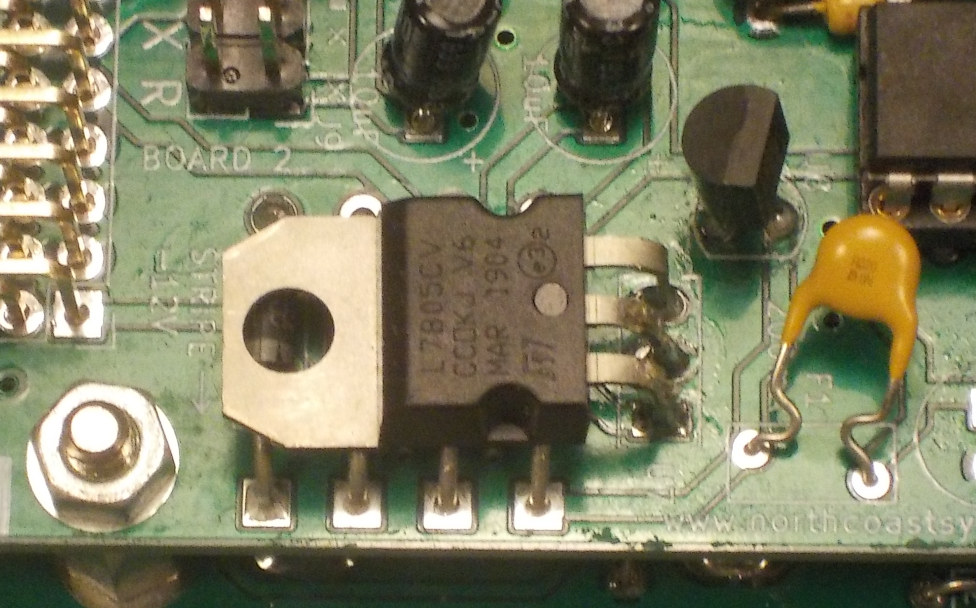
\includegraphics[width=\linewidth]{optional-7805.jpg}\hspace*{\fill}\par} 

The 7805 regulator chip is not included in kits, and adding it is not a
recommended or supported configuration.  Depending on the amount of current
drawn by the external USB device, a 7805 installed as shown without a heat
sink may be liable to overheat.  Using an external device that needs maximum
rated power, or more, for more than a few seconds at a time may necessitate
adding a heat sink to the 7805 chip.  Furthermore, it is possible to set the
configuration jumpers in such a way that the on-board 7805 will be
cross-connected with the Eurorack bus -- meaning that it will attempt to
supply $+$5V power to other modules (possibly useful, but further increasing
the likelihood of overheating), or interfere with the existing bus $+$5V
supply if there is one after all.

The 7805, if installed, will have very little effect unless also activated
with the ``R'' jumper described below, so it remains possible to use a
modified module with bus power instead as long as you are careful with the
jumper configuration.

\section{Bus access and configuration jumpers}

There is a jumper block on the back of the module for selecting the $+$5V
source and whether to connect the first channel (left side of the front
panel) output jacks to the Eurorack bus.
\emph{At least one jumper (the one selecting $+$5V source) must be correctly
installed for the Gracious Host to operate at all.}

\nopagebreak\noindent
{\hspace*{\fill}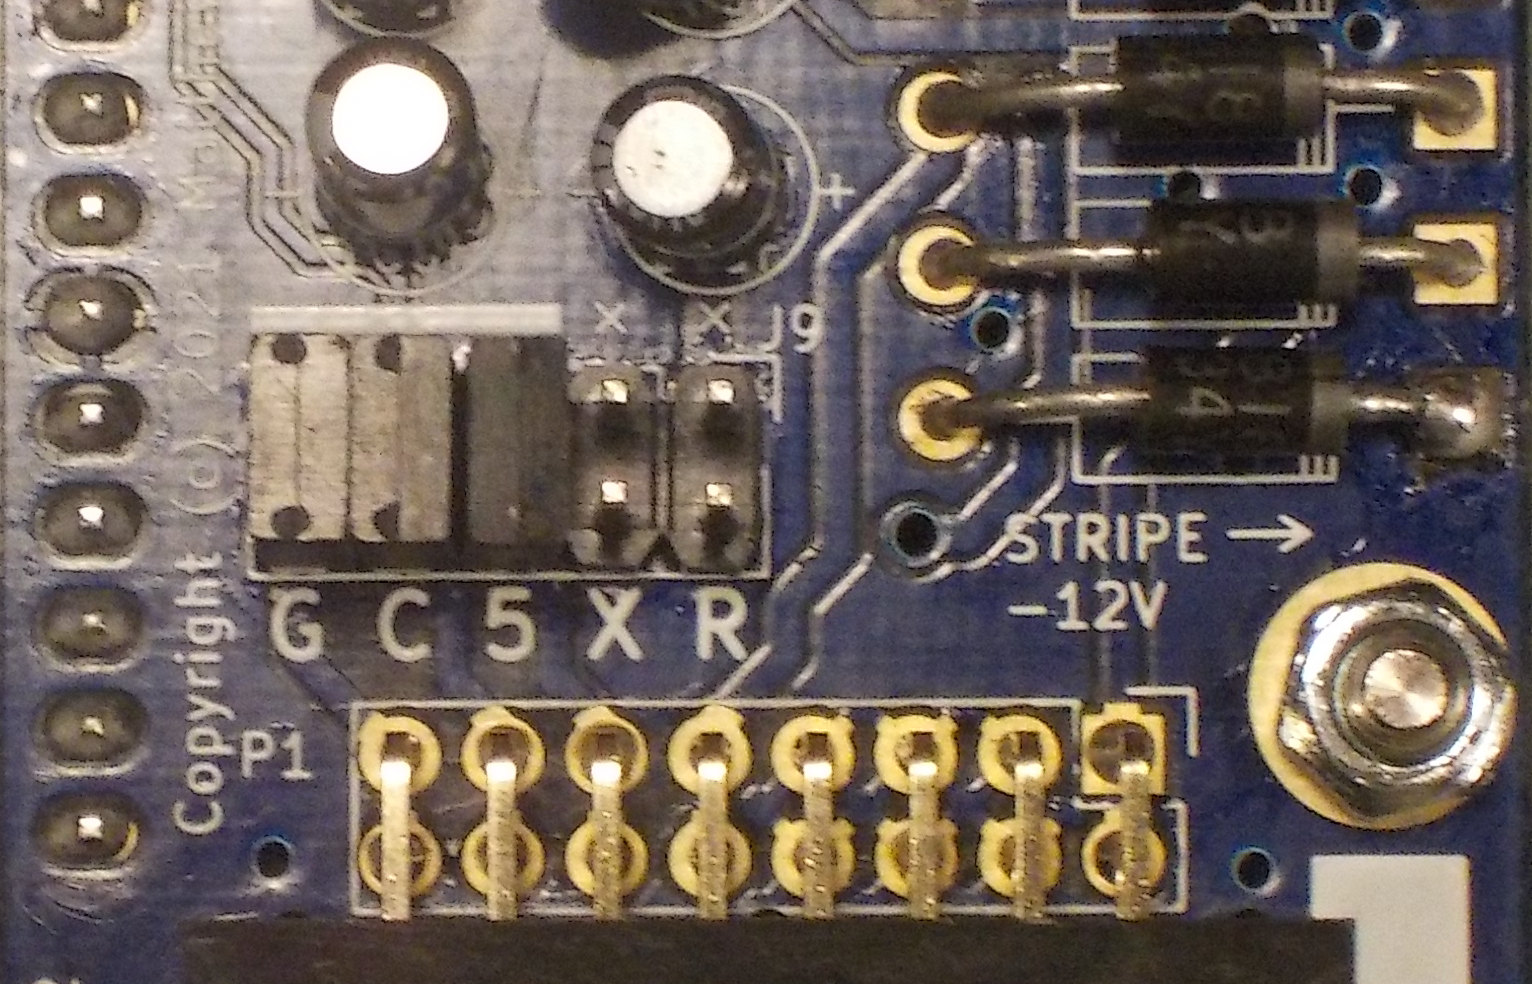
\includegraphics[width=\linewidth]{jumpers.jpg}\hspace*{\fill}\par} 

Left to right, the jumper positions are:
\begin{itemize}
  \item ``G'':  install to connect left GT output to the ``gate'' bus;
  \item ``C'':  install to connect left CV output to the ``pitch CV'' bus;
  \item ``5'':  install to draw $+$5V power from the Eurorack bus;
  \item ``X'':  spare position, no effect; and
  \item ``R'':  install to draw $+$5V power from the onboard regulator, if
    one is installed -- otherwise no effect.
\end{itemize}

Four pins of the standard Eurorack bus are reserved for transmitting pitch
and gate CV among modules.  Most Eurorack cases will connect these pins
among modules -- usually with a separate CV/gate bus for each busboard in
multi-busboard systems.  Some of Doepfer's VCOs, like the A-110-1, receive
pitch CV from the bus by default when no pitch CV is connected to the front
panel, and North Coast's Middle Path VCO (the MSK~013) does the same. 
Modules like the Doepfer A-185-2 are capable of transmitting CV and gate
signals onto the bus.  Some Cwejman, Macbeth, MakeNoise, Malekko, MFB, Plan
B, Synthwerks, TipTop, and other manufacturers' modules also use these pins
in a compatible way.  So with compatible VCOs, you can just plug the
Gracious Host into the same busboard and have it control the VCO pitch
without needing to patch them with front-panel cables.  Similarly, you may
be able to have the gate signal from the Gracious Host activate envelopes or
VCAs without patching.

Some manufacturers have attempted to send digital signals over the CV/gate
bus in a non-standard way under the name ``sync bus.'' Despite more than one
using this name, each manufacturer attempting digital use of the bus has
defined its own nonstandard format for the signals (usually some variation
of MIDI adapted to voltage levels instead of current-loop), and they are not
in general compatible with each other.  Such use also is not compatible with
the analog use of the CV/gate bus as defined by Doepfer, and the two should
not be mixed.

To have the Gracious Host transmit pitch and gate CV onto the bus, install
jumpers in the first two positions, labelled ``G'' and ``C.'' These two
jumpers have the effect of connecting the output jacks directly to the bus. 
It is also possible to install just one of the two jumpers, to transmit only
pitch or only gate CV.  The standard or default configuration for assembled
modules sold by North Coast Synthesis is to install both these jumpers; but
it \emph{will} be necessary to remove them for good results if using more
than one Gracious Host on the same bus.  At most one module on a given
Eurorack bus should be configured to drive the CV/gate bus.  Setting up more
than one module as the bus master is equivalent to patching their outputs
into each other, and is unlikely to work well.

Install a jumper at the third position, labelled ``5,'' to connect the
Gracious Host's internal $+$5V supply to the Eurorack bus.  This should
always be done, for standard unmodified Gracious Host modules.  The only
reason not to install this jumper would be if the module has been modified
with an onboard regulator, in which case you could install the jumper in the
fifth position (``R'') instead, to use the installed onboard regulator.  It
would also be possible to install jumpers at both positions ``5'' and ``R,''
in which case the modified Gracious Host will attempt to regulate $+$12V
power down to $+$5V \emph{and also} supply that power to other modules
through the bus.  Doing so is potentially dangerous, but could possibly be
useful in a very small system where it might be desired to support some
other $+$5V module when the main power supply has no $+$5V rail.

The fourth jumper position (``X'') is unconnected, and the fifth (``R'')
is also unconnected in a standard build.  So, in an unmodified module, these
two jumper positions may be used as storage locations for the two extra
jumpers when CV/gate bus access is \emph{not} desired.  That way, there is
less risk of losing the jumpers.

\section{Source package}

A ZIP archive containing source code for this document and for the module
itself, including things like machine-readable CAD files, is available from 
the Web site at 
\url{https://northcoastsynthesis.com/}.  Be aware that actually building
from source requires some manual steps; Makefiles for GNU Make are provided,
but you may need to manually generate PDFs from the CAD files for inclusion
in the document, make Gerbers from the PCB design, manually edit the .csv
bill of materials files if you change the bill of materials, and so on.

Recommended software for use with the documentation and hardware source code
includes:
\begin{itemize}
  \item GNU Make;
  \item \LaTeX\ for document compilation;
  \item LaTeX.mk (Danjean and Legrand, not to be confused with other
    similarly-named \LaTeX-automation tools);
  \item Circuit\_macros (for in-document schematic diagrams);
  \item Kicad (electronic design automation);
  \item Qcad (2D drafting); and
  \item Perl (for the BOM-generating script).
\end{itemize}

The kicad-symbols/ subdirectory contains my customised schematic symbol and
PCB footprint libraries for Kicad.  Kicad doesn't normally keep dependencies
like symbols inside a project directory, so on my system, these files
actually live in a central directory shared by many projects.  As a result,
upon unpacking the ZIP file you may need to do some reconfiguration of the
library paths stored inside the project files, in order to allow the symbols
and footprints to be found.  Also, this directory will probably contain some
extra bonus symbols and footprints not actually used by this project,
because it's a copy of the directory shared with other projects.

The source package also contains source code for the module firmware, which
is written in PIC24 assembly language and documented in the \emph{MSK~014
Gracious Host Programmer's Manual}.  Working with that code will require
additional software tools -- in particular, Microchip's version of the GNU
assembly language toolchain.

The whole package is covered by the GNU GPL, version 3, a copy of which is
included in the file COPYING.

\section{PCBs and physical design}

The enclosed PCB design is for two boards, each
3.90$''$\linebreak[0]$\times$\linebreak[0]1.50$''$ or
99.06mm\linebreak[0]$\times$\linebreak[0]38.10mm.
The two boards are intended to
mount in a stack parallel to the Eurorack panel, held together with M3
machine screws and male-female hex standoff hardware.  See
Figure~\ref{fig:panel-stack}.  With 12mm of clearance for the power
connector and cable, the module should fit in about 39mm of depth measured from the
back of the front panel.

\begin{figure}
{\centering
\begin{tikzpicture}[scale=0.1]
  % power connector clearance
  \path[draw=black,dashed,thick] (27.2,-54.00) rectangle (39.2,-35.59);
  % panel
  \path[draw=black,fill=black!30!white] (-2.0,-64.25) rectangle (0,64.25);
  % panel-board 1 standoffs
  \path[draw=black,fill=white] (0,-32.93) rectangle (13,-26.93);
  \path[draw=black,fill=white] (0,51.72) rectangle (13,45.72);
  % board 1
  \path[draw=black,fill=blue!50!white] (13,-46.53) rectangle (14.6,52.53);
  % board 1-board 2 standoffs
  \path[draw=black,fill=white] (14.6,-32.93) rectangle (25.6,-26.93);
  \path[draw=black,fill=white] (14.6,51.72) rectangle (25.6,45.72);
  % board 2
  \path[draw=black,fill=blue!50!white] (25.6,-46.53) rectangle (27.2,52.53);
  % nuts and standoff thread ends at back
  \path[draw=black,fill=white] (27.2,-32.93) rectangle (29.2,-26.93);
  \path[draw=black,fill=white] (27.2,51.72) rectangle (29.2,45.72);
  \path[draw=black,fill=black!10!white] (29.2,-30.93) rectangle (31.2,-28.93);
  \path[draw=black,fill=black!10!white] (29.2,49.72) rectangle (31.2,47.72);
  % labels, arrows
  \node at (6.5,38) {\parbox{10mm}{\centering \small 13mm standoff}};
  \node at (20.1,38) {\parbox{11mm}{\centering \small 11mm standoff}};
  \node at (13,64) {\small 2mm front panel};
  \node at (21.4,60.5) {\small 2$\times$ 1.6mm PCBs};
  \draw[>=latex',->,very thick] (13.8,58.7) -- (13.8,53.0);
  \draw[>=latex',->,very thick] (26.4,58.7) -- (26.4,53.0);
  \node at (36.2,-18)
    {\parbox{17mm}{\centering \small 12mm clearance for mated power connector}};
  \draw (39.2,-55) -- (39.2,-64);
  \draw[>=latex',<->,thick] (0,-59.5) -- (39.2,-59.5);
  \node[fill=white] at (20.0,-59.5) {\small $\approx$39mm depth};
\end{tikzpicture}\par}
\caption{Assembled module, side view.}\label{fig:panel-stack}
\end{figure}

\section{Blink codes}

The two bi-colour LEDs on the front panel are used for multiple purposes. 
In most modes they light up in time with the notes being played.  They
flicker briefly when a USB device is inserted, both as a generic indicator
that something is happening, and to support debugging of the stages of the
USB attachment process.  But in some special situations the LEDs display
coded blinking patterns that report the module's status or error condition,
and these patterns are illustrated in this manual with diagrams like the
ones below.  Time reads left to right, with the entire diagram representing
a cycle that repeats every 1.05s.

If a hub is inserted in the USB port -- bearing in mind that the Gracious
Host does not work with hubs -- it will display bursts of four short red
flashes (Morse code ``H'' for ``hub'') on the right LED, leaving the left
LED dark, until the hub is removed.

\nopagebreak
\blinkcodeLR{}{}{}{0/0.5,1/1.5,2/2.5,3/3.5}

For an unsupported device other than a hub, the blink code is similar to the
one for ``hub,'' but the flashes are in a long-short-short pattern; Morse
code ``D'' for ``device unsupported.''

\nopagebreak
\blinkcodeLR{}{}{}{0/1.5,2/2.5,3/3.5}

In the event that something goes wrong inside a per-device USB driver and
the module is unable to recover while the device is attached, it displays
very fast back-and-forth red flashes until the device is removed.

\nopagebreak
\blinkcodeLR{}{0/0.5,1/1.5,2/2.5,3/3.5,4/4.5,5/5.5,6/6.5,7/7.5}%
{}{0.5/1,1.5/2,2.5/3,3.5/4,4.5/5,5.5/6,6.5/7,7.5/8}

If the module gracefully detects a trip of the USB polyfuse, indicating a
short circuit or that someone tried to charge a non-compliant high-power
device through the USB port, then in principle the firmware will try to
display a pattern of mostly red interrupted by short green flashes and
pauses.  Really, though, this display is unlikely to work; in actual testing
of an overloaded port condition the module is often sufficiently messed up
that it shuts off until power-cycled, or at least until the polyfuse cools
down.

\nopagebreak
\blinkcodeLR{3/3.5,5.5/6}{1/3,3.5/5.5,6/8}%
{1.5/2,7/7.5}{0/1.5,2/4,5/7,7.5/8}

There are other blink codes specific to the calibration procedure, which are
illustrated in the section on calibration.

\section{Use and contact information}

This module design is released under the GNU GPL, version 3, a copy of which
is in the source code package in the file named \texttt{COPYING}.  One
important consequence of the license is that if you distribute the design to
others -- for instance, as a built hardware device -- then you are obligated
to make the source code available to them at no additional charge, including
any modifications you may have made to the original design.  Source code for
a hardware device includes without limitation such things as the
machine-readable, human-editable CAD files for the circuit boards and
panels.  You also are not permitted to limit others' freedoms to
redistribute the design and make further modifications of their own.

I sell this and other modules, both as fully assembled products and
do-it-yourself kits, from my Web storefront at
\url{http://northcoastsynthesis.com/}.  Your support of my business is what
makes it possible for me to continue releasing module designs for free. 
The latest version of this document and the associated source files can be
found at that Web site.

Email should be sent to\\ \url{mskala@northcoastsynthesis.com}.
